\documentclass[aspectratio=169,12pt]{beamer}
%	\usetheme{Antibes}
	\usetheme{Frankfurt}

%\usepackage{amsmath}

\usepackage{graphics}
\graphicspath{{../img}}

%\definecolor{VerdeApostila}{rgb}{0.058823529411764705, 0.6862745098039216, 0.30980392156862746}
%\usecolortheme[named=VerdeApostila]{structure}

\newcommand{\modo}[2]{
%	#2
} % claro ou escuro
\newcommand{\quebra}{
	\break
}

\newcommand{\iniciar}[3]{

	\begin{frame}[plain]
		\maketitle
		\centering
		
		\textbf{Aula #1}: 
		#2 
		 
		#3
	  \end{frame}

%	\section*{Nesta aula}
	\begin{frame}{Nesta aula}
		\begin{multicols}{3}
			\tableofcontents
		\end{multicols}	
	  \end{frame}  

}

\newcommand{\terminar}[1]{

\section{Exercícios #1}
\begin{frame}[allowframebreaks]{Exercícios}	% containsverbatim
	\input{aula#1_exercícios}	
  \end{frame}	
  
\section*{}  

\begin{frame}[plain]
	\maketitle
	
	\centering	
	\Large
	\textbf{Dúvidas?}
		
	\url{akira.demenech@uel.br}
  \end{frame}

\end{document}

}

%\usepackage[brazil]{babel}	
%\usepackage[T1]{fontenc}

\usepackage{xcolor}

\usepackage{amsmath}
\usepackage{mathdots}

\usepackage{multicol}

\usepackage{hyperref}
\newcommand{\link}[2]{\href{#1}{\texttt{#2}}}

\title{Minicurso de Python}
\author{Guilherme Akira Demenech Mori}
\date{}

\institute{
%	\link{https://www.facebook.com/codificajr/}{
%		\includegraphics[width=0.3\textwidth]{\modo{Logo pronta.pdf}{logo clara.pdf}}
%	}
}

\begin{document}
	\modo{}{\color{white}}

\iniciar{1}{Variáveis e Operadores}{Dados} 		
		


\section*{Curso}

\begin{frame}{Calendário}	
	\ \vfill					
	\begin{itemize}		
		
		\item[07/04] 
			Dados
			--
			Variáveis e Operações 
			  
			
		\item[09/04]	
			Fluxo 
			--
			Estruturas condicionais e Laços de repetição 
			 
			
		\vfill	
			
		\item[14/04] 
			Funções e Pacotes 
			
		\item[16/04]
			Arquivos 	
			
		\vfill	
			
		\item[\color{purple} 21/04]	
			
		\item[23/04]
			Dúvidas 							
	\end{itemize}
	\vfill	\ 
  \end{frame}

\begin{frame}{Apostila}
	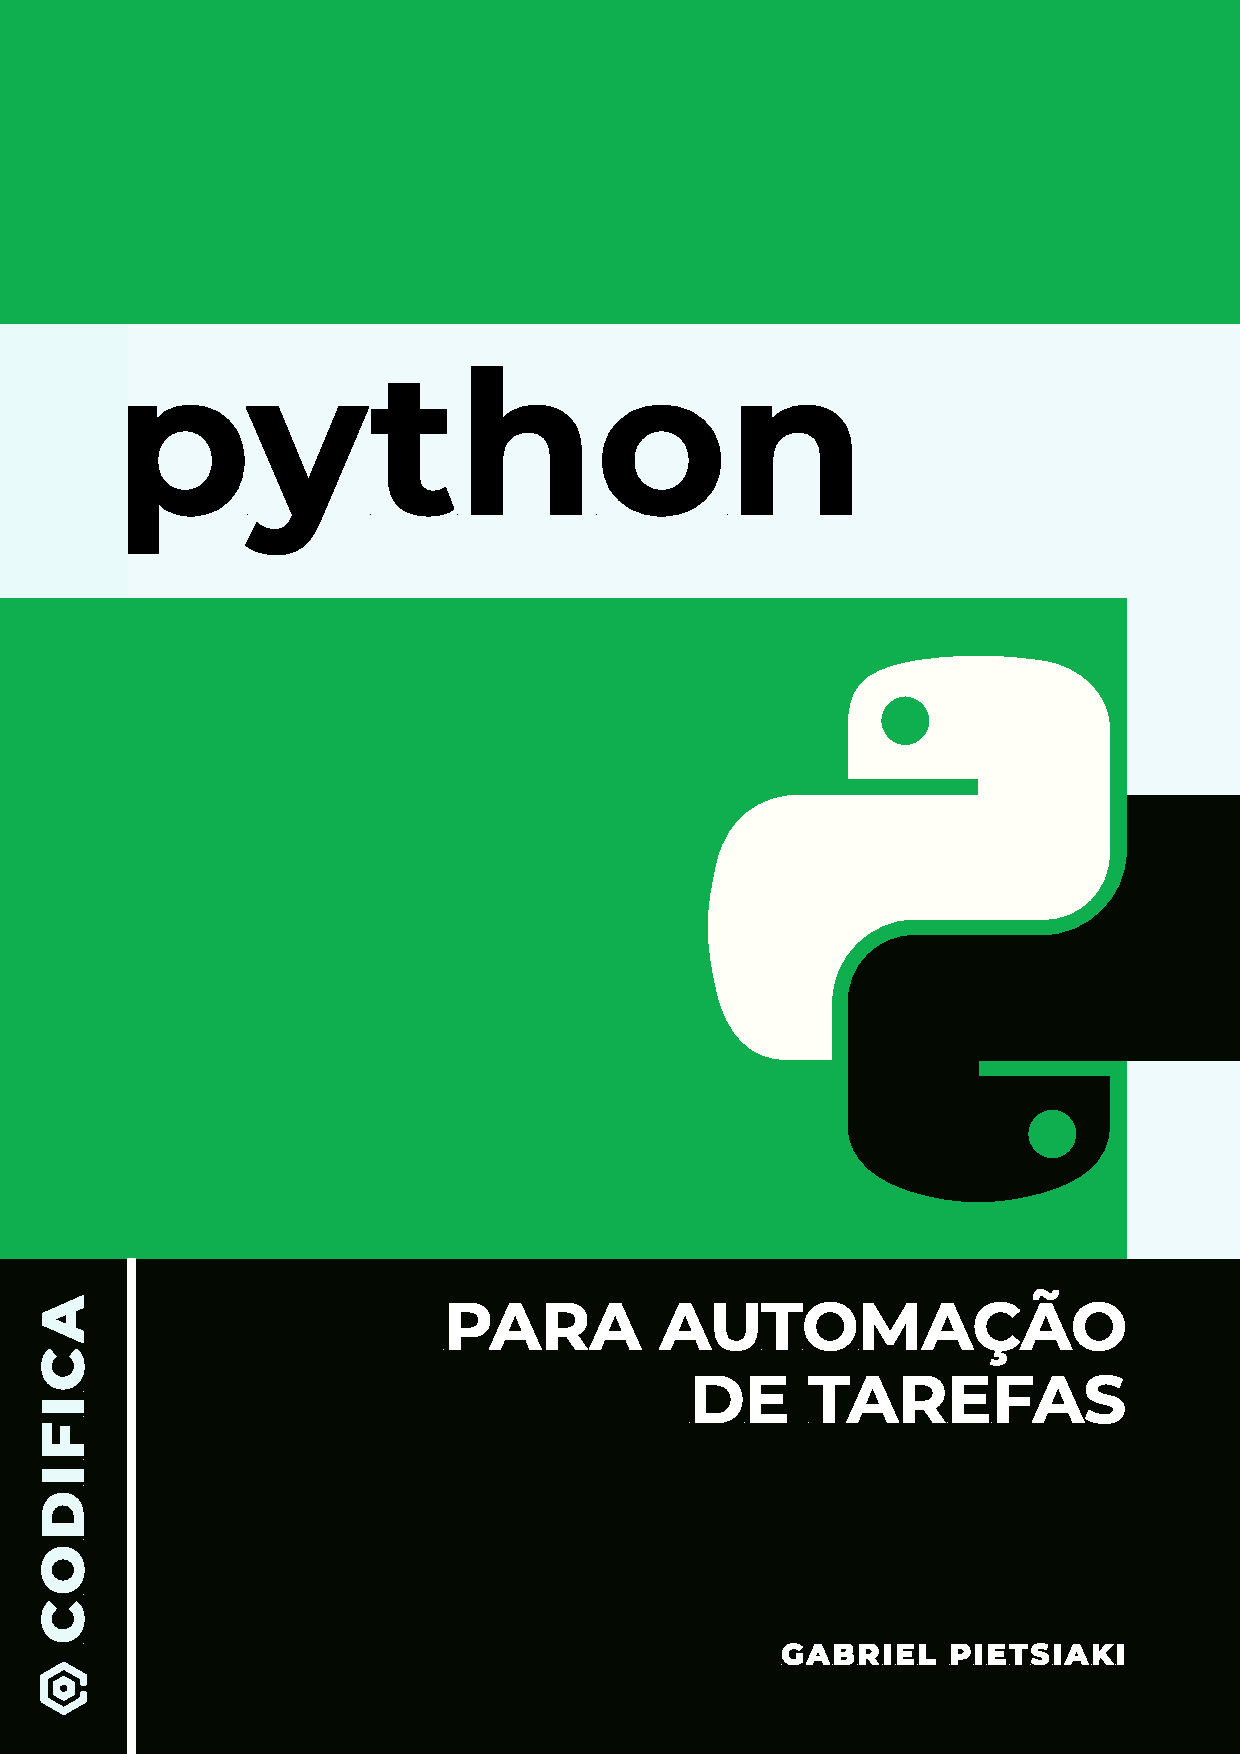
\includegraphics[height=0.7\textheight]{../../APOSTILA-Python-Para-Automação-De-Tarefas.pdf}	
	\hfill	
	
\includegraphics[height=0.7\textheight]{apostila.pdf}
	\hfill
	\ 
	
	\link{https://drive.google.com/file/d/1XX-EbFRS2Og4PDoVmzo5h29ABg-qqiTD/view}{drive.google.com/open?id=1XX-EbFRS2Og4PDoVmzo5h29ABg-qqiTD}	
	 
  \end{frame}

\begin{frame}{Materiais}
	\link{https://github.com/sb-uel/Minicurso-de-Python}{github.com/sb-uel/Minicurso-de-Python}
	
	
\includegraphics[height=0.7\textheight]{github.pdf}
\end{frame}  

\begin{frame}{Redes sociais}
	\huge
	
	\textbf{Instagram}: 
	\link{https://www.instagram.com/ieeeuel/}{@ieeeuel}
	
	\textbf{YouTube}: 	
	\link{https://www.youtube.com/@RamoIEEEUEL}{@RamoIEEEUEL}
\end{frame}

	

\section*{Introdução}

\begin{frame}{O que é Python?}
	
	Python é uma linguagem de programação muito versátil 
	\hfill 
	
\includegraphics[width=0.3\textwidth]{python.pdf}
	
%	\begin{multicols}{2}			
	\begin{itemize}
		\item \textbf{de alto nível}:
			mais abstração, mais próxima do pensamento humano 
			
			
		\item \textbf{multiparadigma}:
			mescla aspectos de vários paradigmas de programação 
		
		\vfill
		
		\item \textbf{interpretada}:
			é executada por um interpretador diretamente a partir do código fonte 
			
		\item \textbf{de script}: 
			é executada à medida que é lida, linha a linha
		
		\vfill	
			
%		\item imperativa
		
		\item \textbf{fortemente tipificada}:
			os dados são obrigados a seguir tipos rígidos 
			
		\item \textbf{dinamicamente tipificada}:	
			variáveis podem ser atribuídas a dados de tipos diferentes
	\end{itemize}
%	\end{multicols}
\end{frame}

%\begin{frame}{Python e Eu}
%	2017--2018
%  \end{frame}

\subsection{Instalação}
\begin{frame}{Como instalar}%[allowframebreaks]	
	Instale o interpretador de Python para executar os programas:

%	Interpretador 
\textbf{Python}:	\link{https://www.python.org/}{python.org}  

ou escolha uma versão na Microsoft Store:  

\link{https://apps.microsoft.com/search/publisher?name=Python+Software+Foundation}{apps.microsoft.com/search/publisher?name=Python+Software+Foundation}
% PSF https://apps.microsoft.com/search/publisher?name=Python+Software+Foundation
% 3.10 https://www.microsoft.com/store/productId/9PJPW5LDXLZ5
% 3.11 https://www.microsoft.com/store/productId/9NRWMJP3717K?ocid=pdpshare 
% 3.12 https://www.microsoft.com/store/productId/9NCVDN91XZQP

\vfill

Escolha uma IDE para escrever os programas:
\begin{itemize}
	\item 
	\textbf{VS Code}:	
	\link{https://code.visualstudio.com/}{code.visualstudio.com}
	
	ou na Microsoft Store:  \link{https://apps.microsoft.com/store/detail/XP9KHM4BK9FZ7Q}{apps.microsoft.com/store/detail/XP9KHM4BK9FZ7Q}
	
	\item 
	\textbf{PyCharm}: 	
	\link{https://www.jetbrains.com/pt-br/pycharm/}{jetbrains.com/pycharm}
	
	\vfill
	
%	\item 
%	\textbf{Atom}:
%	\link{https://atom-editor.cc/}{atom-editor.cc}
	
	\item 
	\textbf{Notepad++}:
	\link{https://notepad-plus-plus.org/downloads/}{notepad-plus-plus.org}
	
%	\item
%	\textbf{BowPad}:
%	\link{https://tools.stefankueng.com/BowPad.html}{tools.stefankueng.com/BowPad.html}
\end{itemize}						
  \end{frame}

\begin{frame}
	Ou edite e execute online, sem instalar nada: \hfill {\color{red} \footnotesize não recomendado para manipulação de arquivos}

\begin{enumerate}
	\item 
	\textbf{Google Colab}: 
	\link{https://colab.research.google.com/}{colab.research.google.com}
	(necessário login no \textit{Gmail})
	
	\item
	\textbf{W3Schools Python Compiler (Editor)}: \\
	\link{https://www.w3schools.com/python/trypython.asp?filename=demo_syntax_variables}{w3schools.com/python/trypython.asp?filename=demo\_compiler}				
	
	\item
	\textbf{Online Python IDE}:
	\link{https://www.online-python.com/}{online-python.com}
	
	\item
	\textbf{OnlineGDB Python Interpreter}: \\ 
	\link{https://www.onlinegdb.com/online_python_interpreter}{onlinegdb.com/online\_python\_interpreter}
	
	\item
	\textbf{Programiz online compiler (interpreter)}: \\ 
	\link{https://www.programiz.com/python-programming/online-compiler/}{programiz.com/python-programming/online-compiler}
	
	\item 
	\textbf{Tutorials Point Online Python Compiler}: \\ 
	\link{https://www.tutorialspoint.com/python/online-python-compiler.php}{tutorialspoint.com/python/online-python-compiler.php}
	
	\item
	\textbf{GeeksforGeeks Python Online Compiler}: \\ 		
	\link{https://ide.geeksforgeeks.org/online-python-compiler}{ide.geeksforgeeks.org/online-python-compiler}
	
	\vfill
	....
\end{enumerate}
  \end{frame}  

\frame{Se quiser utilizar no smartphone, há várias opções.

\begin{enumerate}
	
	\item \textbf{Pydroid}: 
	\link{https://play.google.com/store/apps/details?id=ru.iiec.pydroid3&hl=pt_BR}{play.google.com/store/apps/details?id=ru.iiec.pydroid3}
	
	\item \textbf{QPython}:
	\link{https://play.google.com/store/apps/details?id=org.qpython.qpy}{play.google.com/store/apps/details?id=org.qpython.qpy}
	
\end{enumerate}}


\section{Variáveis e valores} % variáveis e valores 

\begin{frame}{O que é uma variável?}
	Variável é um nome ao qual pode ser atribuído um valor.	
	
	Depois, pode ser atribuído outro valor.
	
	\vfill	
	
	O nome deve começar com uma letra maiúscula, minúscula ou com \texttt{\_} (underline)
	e o resto do nome pode conter letras maiúsculas, minúsculas, \texttt{\_} (underline) ou dígitos.
	
	Não são permitidos espaços, \texttt{-} (traço), \texttt{.} (ponto), \texttt{/} (barra) ou outros símbolos dentro do nome de uma variável.

	\vfill
	
	\textbf{Nomes válidos}: \texttt{a}, \texttt{A}, \texttt{abacaxi}, \texttt{x1}, \texttt{t\_0}, \texttt{\_b2C}....	
	
	\textbf{Nomes ilegais}: \texttt{10}, \texttt{a-x}, \texttt{2b}, \texttt{C\$\_}
	
  \end{frame}	
  
\begin{frame}[containsverbatim]{Como criar uma variável e atribuir um valor a ela}
	\large
	
	Em Python, a variável é criada quando o nome dela recebe um valor pela primeira vez.
	
	Para atribuir um valor para uma variável, basta fazer:
	
	\texttt{nomevariavel = valor}
	\hfill 
	\#
	Essa linha se lê \textit{nomevariavel recebe valor}
  \end{frame}  
  
\begin{frame}[containsverbatim]
\textbf{Exemplos}:
	\Large
	%	\begin{multicols}{2}				
		\begin{verbatim}
			a = 10	# a recebe 10			
			abacaxi = 'oi'	# abacaxi recebe 'oi'									
			x1 = 9.8 # x1 recebe 9.8
		\end{verbatim}					
		%	\end{multicols}
\end{frame}  

\begin{frame}[containsverbatim]
	\Large	
	
	\textbf{Atenção}: 
	não é permitido atribuir da esquerda para a direita, a variável deve estar na esquerda.   
		
	\textbf{Não faça}:
	\begin{verbatim}
		10 = a 	
		'oi' = abacaxi 
	\end{verbatim}	
\end{frame}

% utilizar e reatribuir 
\begin{frame}[containsverbatim]{Como utilizar e atribuir novo valor a uma variável}
	A partir do momento que uma variável existe, ela pode ser utilizada para representar o valor que foi atribuído a ela em qualquer operação (inclusive para atribuir o valor a outra variável).
	
	\textbf{Exemplo}:	
		\begin{verbatim}
			t_0 = x1	# t_0 recebe o valor de x1 (9.8)			
			abacaxi = 'tchau'	# abacaxi recebe 'tchau'												
			x1 = 10	# x1 recebe 10
		\end{verbatim}	
  \end{frame}	
  
\frame{ % atenção
	\large
	\textbf{Atenção}: ao atribuir novo valor para uma variável, quaisquer outras variáveis que tenham recebido o antigo valor dela \textbf{continuam} com o valor antigo.	
	
	A variável também pode receber um novo valor de outro tipo.
}  

\section{Tipos de dados e operações}

\subsection{Dados simples}
\begin{frame}{Tipos de dados simples}% tipos de dados simples 		
		
	\begin{multicols}{2}			
	\begin{itemize}%[<>]
		
		\item \textbf{int}:
			\\ \texttt{10}
			\\ \texttt{-2}
			
		\item \textbf{float}:	
			\\ \texttt{10.0}
			\\ \texttt{-2.0}
			\\ \texttt{9.8}
			\\ \texttt{0.3}
			
		\item \textbf{complex}:	
			\\ \texttt{1j}
			\\ \texttt{3-2j}
			\\ \texttt{4+6j}
			\\ \texttt{-5j}
			\\ \texttt{7.0+0j}
		
		\vfill	
			
		\item \textbf{bool}:	
			\texttt{True}
			ou 
			\texttt{False}
			
		\item \textbf{NoneType}:	
			\texttt{None}
			
%		\vfill 	
		
	\end{itemize}
	\end{multicols}
	
	{\color{purple} são todos imutáveis}
  \end{frame}

\begin{frame}{Operações}
	Para os tipos numéricos 
	(\textbf{int}, \textbf{float} e \textbf{complex}):
	
	\begin{multicols}{2}
		\begin{itemize}
			\item \textbf{Adição}: 
				\texttt{x + y} 
				
			\item \textbf{Subtração}: 
				\texttt{x - y}
				
			\item \textbf{Multiplicação}: 
				\texttt{x * y}	
				
			\item \textbf{Divisão}: 
				\texttt{x / y}	
				
			\item \textbf{Divisão euclidiana}: 
				\texttt{x // y}	
				
			\item \textbf{Módulo}: 
				\texttt{x \% y}	
				
			\item \textbf{Potenciação}: 
				\texttt{x ** y}	
				
			\item \textbf{Inversão}: 
				\texttt{-x}	
		\end{itemize}	
	\end{multicols}	
	
	\vfill
	
	Para o tipo booleano (\textbf{bool}):	
	
	\begin{multicols}{2}
		\begin{itemize}
			\item \textbf{E lógico}: 
				\texttt{x and y} 
			
			\item \textbf{OU lógico}: 
				\texttt{x or y}
			
			\item \textbf{NÃO lógico}: 
				\texttt{not x}								
		\end{itemize}	
	\end{multicols}
	
  \end{frame}	

\subsection{Dados compostos} 
\begin{frame}[containsverbatim]{Tipos de dados compostos}% tipos de dados compostos 
	\begin{itemize}%[<>]			
		\begin{multicols}{3}	
			
			\item \textbf{str}: 
			{\color{purple} é imutável}
\begin{verbatim}
'oi'
'Olá, mundo!'
"Hello, world!"
'A'
''
\end{verbatim}

			\vfill
			
			\item \textbf{list}:	
			permite edição
\begin{verbatim}
[10, -2]
[10.0, -2.0, 9.8]
['oi', 0.3, False]
[-2]
[]
\end{verbatim}			
			
			\vfill
			
			\item \textbf{tuple}: 
			{\color{purple} é imutável}	 
\begin{verbatim}
(10, -2)
(10.0, -2.0, 9.8)
('oi', 0.3, False)	
(-2,)	
()	
\end{verbatim} 	
			
		
		\end{multicols}
	\end{itemize}	
  \end{frame}
  
\begin{frame}[containsverbatim]			
\begin{itemize}	
\item \textbf{dict}: 
	{\color{red} só aceita chaves imutáveis}, 
	permite edição de si e dos seus valores 
	\begin{verbatim}
		{10: 0, -2: 3}
		{'a': 10.0, '4': -2.0, 'chave composta': 9.8}
		{'oi': [-2], 0.3: None, False: {10: 0, -2: 3}}
		{-2: 3}
		{} # não confunda com o conjunto vazio
	\end{verbatim} 
\end{itemize}
\end{frame}  

\begin{frame}[containsverbatim]			
	\begin{itemize}		
		\item \textbf{set}: 
		{\color{red} só aceita valores imutáveis}  
		e permite edição 
		\begin{verbatim}
			{10, -2}
			{10.0, -2.0, 9.8}
			{'oi', 0.3, False}
			{-2}
			set()	# não confunda com o dicionário vazio
		\end{verbatim}
	\end{itemize}
\end{frame}

\begin{frame}{Operações}
	Para tipos compostos sequenciais 
	(\textbf{str}, \textbf{tuple} e \textbf{list}):
	\begin{multicols}{2}
		\begin{itemize}	
			\item \textbf{Concatenação}: 
				\texttt{v + u} 
				
			Some os dados (precisam ser do mesmo tipo) para que um composto maior seja criado 	
			
			\item \textbf{Repetição}: 
				\texttt{v * x}									
				
			Multiplique os dados por um \textbf{int} para que sejam repetidos essa quantidade de vezes.	
		\end{itemize}				
	\end{multicols}	
 \end{frame}

% acessando e manipulando dados compostos 
\begin{frame}[containsverbatim]{Acessando e manipulando dados compostos} 
	Acessar valor a partir do índice 
	(\textbf{str}, \textbf{tuple} e \textbf{list}):
	\texttt{nomevariavel[indice]}
	
	\# o índice começa no 0
	
\begin{verbatim}
	abacaxi[0]
	abacaxi[1]
\end{verbatim}	
	
  \end{frame}	

\begin{frame}[containsverbatim]
	Gerar novo composto a partir de intervalo
	(\textbf{str}, \textbf{tuple} e \textbf{list}):
	\texttt{nomevariavel[inicio:fim]}
	
	\begin{verbatim}
		A[2:5]	
	\end{verbatim}
\end{frame}

\begin{frame}[containsverbatim]
	Atribuir novo valor num índice 
	(\textbf{list}):
	\texttt{nomevariavel[indice] = novovalor}
	
	\# o índice já deve ter algum valor
	
	\begin{verbatim}
		A[1] = 'Olá, mundo!' 	
	\end{verbatim}	
\end{frame}

\begin{frame}[containsverbatim]
	Adicionar novo valor ao final da lista 
	(\textbf{list}):
	\texttt{nomevariavel.append(novovalor)}	
	
	\begin{verbatim}
		A.append("Hello, world!") 	
	\end{verbatim}
\end{frame}

\begin{frame}[containsverbatim]
	Adicionar novo valor ao final do conjunto 
	(\textbf{set}):
	\texttt{nomevariavel.add(novovalor)}	
	
	\begin{verbatim}
		X.add(10) 	
	\end{verbatim}
	
\end{frame}

\begin{frame}[containsverbatim]
	Remover o primeiro valor do conjunto 
	(\textbf{set}):
	\texttt{nomevariavel.pop()}	
\end{frame}

\begin{frame}[containsverbatim]
	Remover o último valor da lista 
	(\textbf{list}):
	\texttt{nomevariavel.pop()}	
	
	Remover valor da lista pelo índice
	(\textbf{list}):
	\texttt{nomevariavel.pop(indice)}	
\end{frame}

\begin{frame}[containsverbatim]
	Quantidade de valores 
	(\textbf{str}, \textbf{tuple}, \textbf{list}, \textbf{set}, \textbf{dict}):
	\texttt{len(nomevariavel)}
	
	\begin{verbatim}
		len(abacaxi)
		len(A)
		len(X)
		len(f) 	
	\end{verbatim}
\end{frame}

\begin{frame}[containsverbatim]
	Acessar valor a partir da chave 
	(\textbf{dict}):
	\texttt{nomevariavel[chave]}
	
	\begin{verbatim}
		f[10]
		f[-2]
		h['oi']
		h[0.3]
		h[False]
	\end{verbatim}
\end{frame}

\begin{frame}[containsverbatim]
	Atribuir novo valor numa chave 
	(\textbf{dict}):
	\texttt{nomevariavel[chave] = novovalor}
	
	\begin{verbatim}
		g['a'] = True
		g['4'] = 'Olá, mundo!'
	\end{verbatim}	
	
\end{frame}

%\begin{frame}[containsverbatim]
%	
%\end{frame}
%
%\begin{frame}[containsverbatim]
%
%\end{frame}

\subsection{Conversão}
% conversão 
\begin{frame}[allowframebreaks]{Convertendo dados}
	\begin{itemize}
		\item \texttt{int(nomevariavel)} converte para \textbf{int}
			\\ \textbf{str} terá o valor inteiro lido (se houver)
			\\ \textbf{float} irá cortar as casas fracionárias (sem arredondar)					
			\\ \textbf{Exemplo}:
			\texttt{int(x1)}			
		
%		\vfill
		
		\item \texttt{float(nomevariavel)} converte para \textbf{float}
			\\ \textbf{str} terá o valor de ponto flutuante lido (se houver)
			\\ \textbf{int} irá adicionar \texttt{.0} 					
			\\ \textbf{Exemplo}:
			\texttt{float(a)}
		
		\quebra
%		\vfill
		
		
		\item \texttt{bool(nomevariavel)} converte qualquer tipo de dados para \textbf{bool}
			\\ Será \texttt{False} se o dado for igual a \texttt{0}, \texttt{None} ou for composto vazio (sem nenhum valor)  					
			\\ Será \texttt{True} se o dado for diferente de \texttt{0} e de \texttt{None} ou for composto não-vazio (pelo menos um valor)
			\\ \textbf{Exemplo}:
			\texttt{bool(abacaxi)}
				
		\quebra
%		\vfill		
		
		\item \texttt{str(nomevariavel)} converte qualquer tipo de dado para sua representação em \textbf{str} 
		
%		\vfill 
		
		\item \texttt{tuple(nomevariavel)}, \texttt{list(nomevariavel)} e \texttt{set(nomevariavel)} convertem dados compostos para os tipos \textbf{tuple}, \textbf{list} e \textbf{set}, respectivamente.
	\end{itemize}
  \end{frame}	

\section{Entrada e saída}
% print 
\begin{frame}[containsverbatim]{Saída de dados}
	\begin{itemize} 	
		\item \texttt{print(valor)} exibe o valor, que pode ser representado por uma variável, pode ser resultado de operações
		
		\item \texttt{print(valor1, valor2, valor3)} permite exibir vários valores (podem ser de tipos diferentes)				
		
	\end{itemize}		 	  
  \end{frame}
  	
\begin{frame}[containsverbatim]{Saída formatada}
\begin{itemize}	
	\item Você pode inserir valores (variáveis, literais ou operações) com formatação de \textbf{str}:

\begin{verbatim}
	print(f'Texto formatado com {valor} dentro')
	print('Texto formatado com str %s dentro' %valors)
	print('Texto formatado com int %d dentro' %valori)
	print('Texto formatado com float %f dentro' %valorf)
\end{verbatim}	

	\item Use concatenação e conversão também, se quiser: 

\begin{verbatim}
	print('Primeira parte ' + 'segunda parte ' + str(valor))
\end{verbatim}	
\end{itemize}	
  \end{frame}

% input 
\begin{frame}[containsverbatim]{Entrada de dados}	
	\begin{itemize}	
		\item Você pode receber dados em forma \textbf{str} (uma linha digitada pelo usuário):
		
\begin{verbatim}
	nomevariavel = input()
\end{verbatim}	
	
	\vfill
		
		\item É possível inserir um texto para pedir a entrada: 
		
\begin{verbatim}
	nomevariavel = input('Escreva uma linha (e pressione enter): ')
\end{verbatim}	

	\vfill 
	
		\item Converta os dados caso você queira outros tipos de entrada:
		
\begin{verbatim}
	nomevariaveli = int(input('Escreva um inteiro dê enter: '))
	nomevariavelf = float(input('Escreva um inteiro e dê enter: '))
\end{verbatim}		
		
	\end{itemize}	
  \end{frame}
 


\terminar{1}
